\usepackage{graphicx}
\usepackage{subcaption} % para grupos de figuras
\usepackage{amssymb} % mas simbolos
%Ej5.1
\subsection{}

%Ej5.2
\subsection{Verificación de $z^{NR}$}
En la tabla \ref{tab:table_5_2} se muestra la norma de $F(z)$ para distintos valores de dimension $n$.

\begin{table}[h!]
    \begin{center}
      \caption{Your first table.}
      \label{tab:table1}
      \begin{tabular}{l|c|r} % <-- Alignments: 1st column left, 2nd middle and 3rd right, with vertical lines in between
        \textbf{n} & \textbf{$||F(z^{NR})||$}\\
        \hline
         100 & 3.574573332905249e-014\\
         200 & 1.175361818307876e-013\\
         300 & 1.997171185243193e-013\\
         400 & 3.256674181109525e-013\\
         500 & 4.902233609479727e-013\\
        1000 & 1.403048923326327e-012\\
        2000 & 3.877314569665418e-012\\
        3000 & 7.960022321886946e-012\\
        4000 & 1.081169278301875e-011\\
        5000 & 1.555144859221123e-011\\
        \hline
      \end{tabular}
    \end{center}
  \end{table}  

Se puede ver que para todos los tamaños, se llega casi a anular la función en 20 iteraciones.

%Ej5.3
\subsection{Tiempo de ejecución de NR2}
Con el fin de estudiar el tiempo de ejecución del algoritmo de NR2, se lo aplica para distintos valores de dimension $n$.
\begin{equation*}
    n = [1, 2, 3, 4, 5, 10, 20, 30, 40, 50] \times 100
\end{equation*}
A continuación se muestran los resultados:
\begin{figure}[h!]
    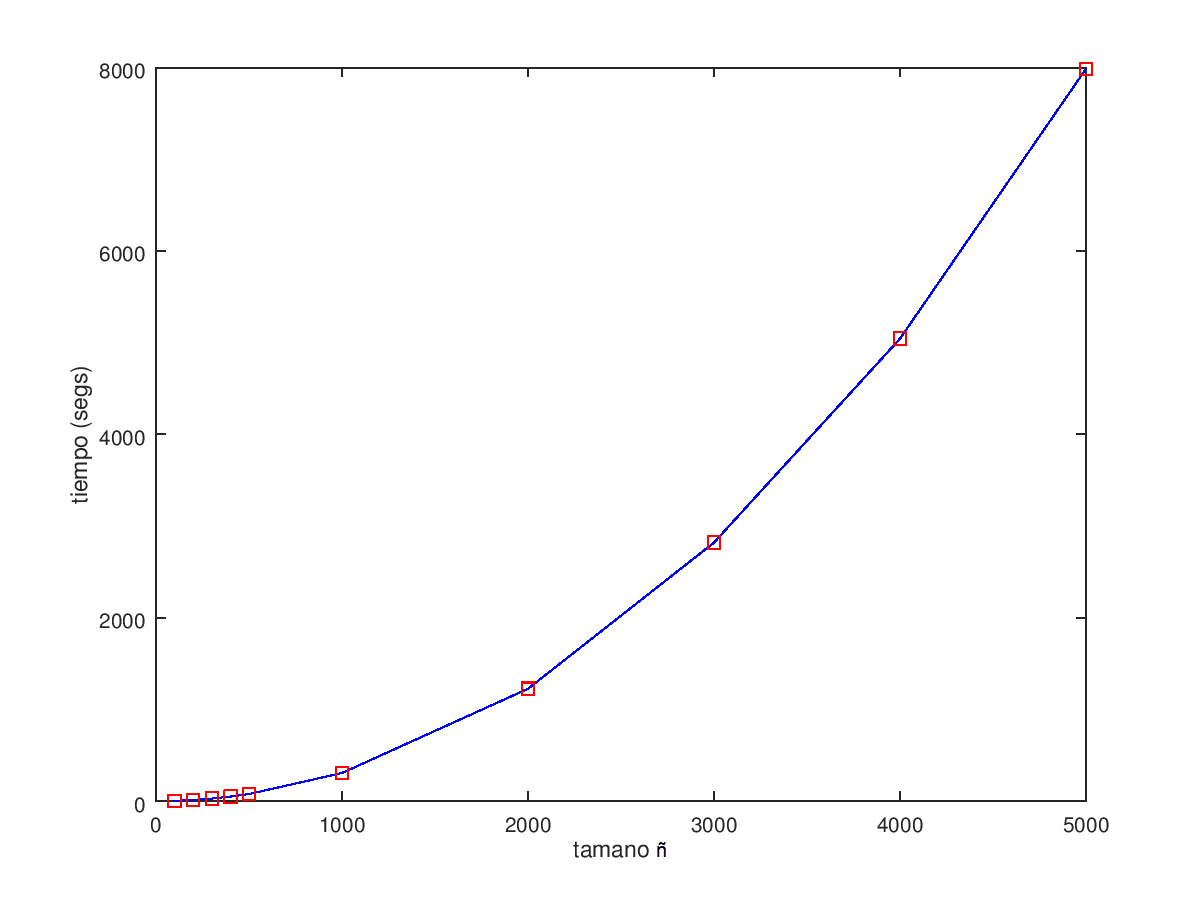
\includegraphics[width=\linewidth]{Grafica_5_3_1.png}
    \caption{Tiempo de ejecución del algoritmo NR2.}
    \label{fig:Grafica_5_3_1}
\end{figure}

\begin{figure}[h!]
    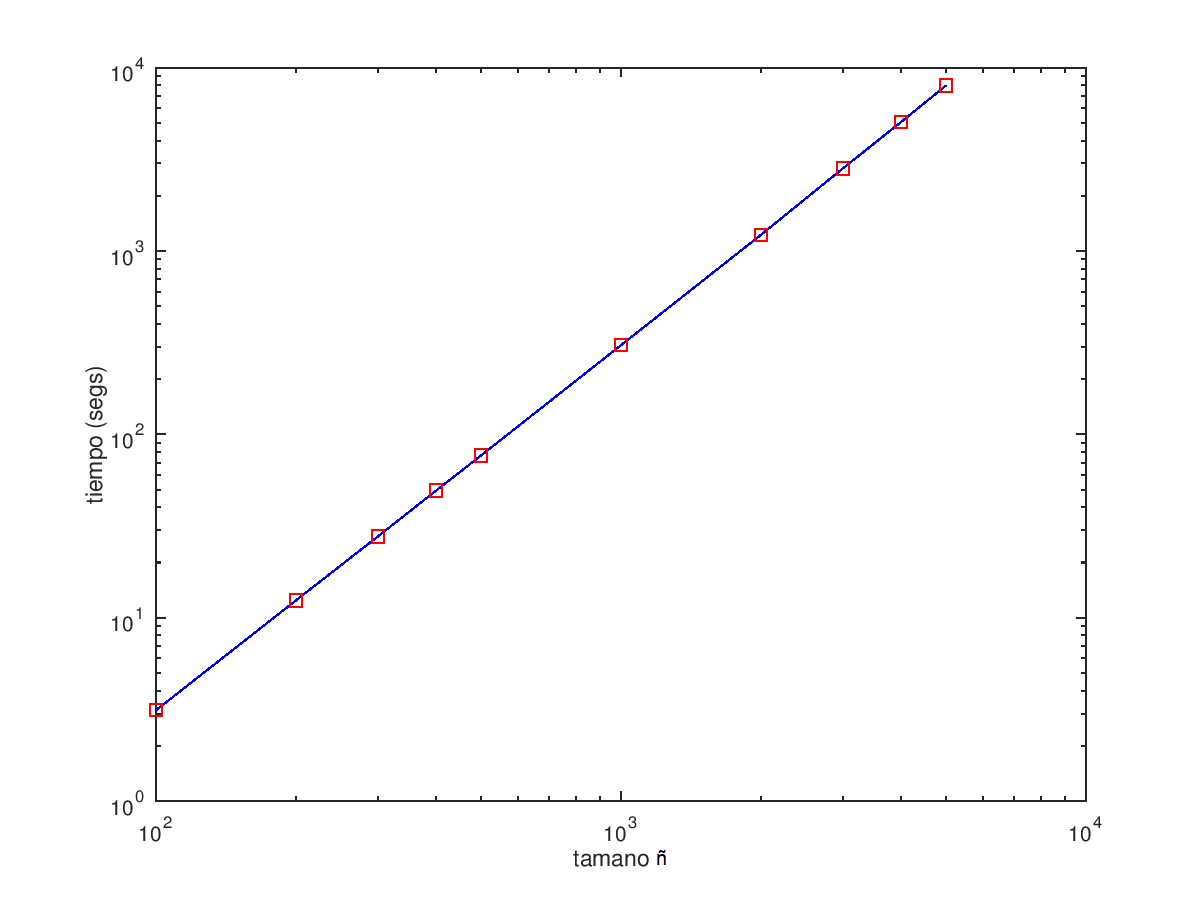
\includegraphics[width=\linewidth]{Grafica_5_3_2.png}
    \caption{Tiempo de ejecución del algoritmo NR2 en escala logaritmica.}
    \label{fig:Grafica_5_3_2}
\end{figure}
En la figura \ref{fig:Grafica_5_3_2}, se puede ver un comportamiento lineal de los datos.
Esto concuerda con lo visto en la sección 4.5, donde se vio que el tiempo de ejecucion es $O(n^2)$.
Comprobemoslo:
\begin{align}
    T(n) &= kn^2 \\
    log(kn^2) &= log(k) + 2log(n) \\
    \text{ C.V.}& \rightarrow y = log(kn^2) \text{ ; } x = log(n) \\
    y &= a + bx
\end{align}

%Ej5.4
\subsection{Ajuste polinomial del tiempo de ejecución}
Utilizando la funcion polyfit de Octave, se ajustan los datos de la sección 5.3 con un polinomio de grado 2.
\begin{figure}[h!]
    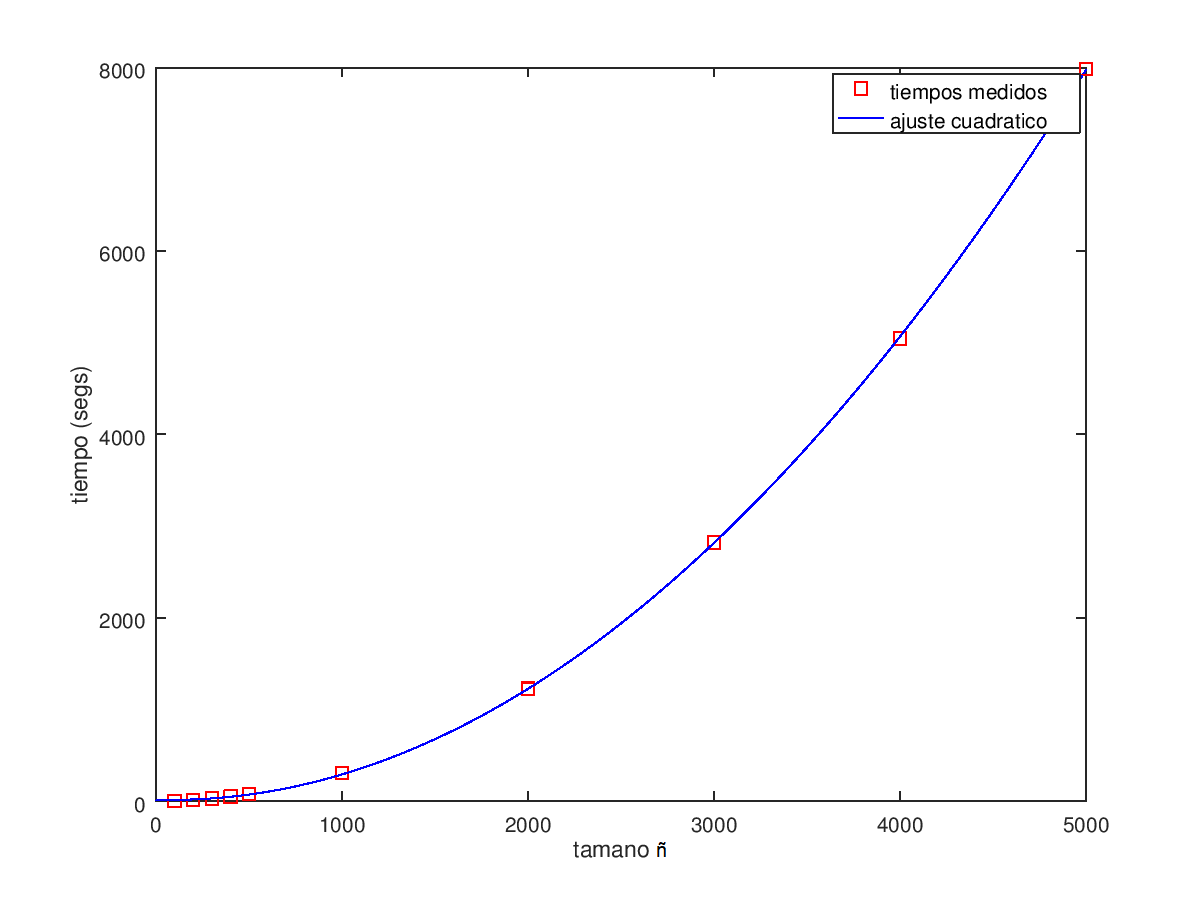
\includegraphics[width=\linewidth]{Grafica_5_4.png}
    \caption{Ajuste cuadratico del tiempo de ejecucion de NR2.}
    \label{fig:Grafica_5_4}
\end{figure}
Como se ve en la figura, con un polinomio de grado 2 se logran ajustar correctamente los datos.
